\documentclass[aspectratio=169]{beamer}
\usetheme{Bruno}
\usepackage{amsmath}
\usepackage{amssymb}
\usepackage{siunitx}
\usepackage{float}
\usepackage{tikz}
\def\checkmark{\tikz\fill[scale=0.4](0,.35) -- (.25,0) -- (1,.7) -- (.25,.15) -- cycle;} 
\usepackage{url}
\usepackage[siunitx,american,RPvoltages]{circuitikz}
\ctikzset{capacitors/scale=0.7}
\ctikzset{diodes/scale=0.7}
\usepackage{tabularx}
\newcolumntype{C}{>{\centering\arraybackslash}X}
\renewcommand\tabularxcolumn[1]{m{#1}}% for vertical centering text in X column
\usepackage{tabu}
\usepackage[spanish,es-tabla,activeacute]{babel}
\usepackage{babelbib}
\usepackage{booktabs}
\usepackage{pgfplots}
\usepackage{hyperref}
\hypersetup{colorlinks = true,
            linkcolor = black,
            urlcolor  = blue,
            citecolor = blue,
            anchorcolor = blue}
\usepgfplotslibrary{units, fillbetween} 
\pgfplotsset{compat=1.16}
\usepackage{bm}
\usetikzlibrary{arrows, arrows.meta, shapes, 3d, perspective, positioning,mindmap,trees,backgrounds}
\renewcommand{\sin}{\sen} %change from sin to sen
\usepackage{bohr}
\setbohr{distribution-method = quantum,insert-missing = true}
\usepackage{elements}
\usepackage{verbatim}
\usepackage[edges]{forest}
\usepackage{etoolbox}
\usepackage{schemata}
\usepackage{appendix}
\usepackage{listings}

\definecolor{color_mate}{RGB}{255,255,128}
\definecolor{color_plas}{RGB}{255,128,255}
\definecolor{color_text}{RGB}{128,255,255}
\definecolor{color_petr}{RGB}{255,192,192}
\definecolor{color_made}{RGB}{192,255,192}
\definecolor{color_meta}{RGB}{192,192,255}
\newcommand\diagram[2]{\schema{\schemabox{#1}}{\schemabox{#2}}}

\definecolor{codegreen}{rgb}{0,0.6,0}
\definecolor{codegray}{rgb}{0.5,0.5,0.5}
\definecolor{codepurple}{rgb}{0.58,0,0.82}
\definecolor{backcolour}{rgb}{0.95,0.95,0.92}

\lstdefinestyle{mystyle}{
    backgroundcolor=\color{backcolour},   
    commentstyle=\color{codegreen},
    keywordstyle=\color{magenta},
    numberstyle=\tiny\color{codegray},
    stringstyle=\color{codepurple},
    basicstyle=\ttfamily\footnotesize,
    breakatwhitespace=false,         
    breaklines=true,                 
    captionpos=b,                    
    keepspaces=true,                 
    numbers=left,                    
    numbersep=5pt,                  
    showspaces=false,                
    showstringspaces=false,
    showtabs=false,                  
    tabsize=2
}

\lstset{style=mystyle}
\title{Instrumentación I: \\ \emph{Mediciones de}\\ \emph{Temperatura}}
\author{
    Juan J. Rojas, Hugo Sanchez Ortiz
}
\institute{Instituto Tecnológico de Costa Rica}
\date{\today}
\background{fig/background.jpg}
\begin{document}
\sisetup{unit-math-rm=\mathrm,math-rm=\mathrm} % change sinitx font
\sisetup{output-decimal-marker = {,}}
\maketitle

\newcommand{\blackandwhite}{white} %change this at the end

\begin{frame}{Definición de Temperatura}
    \begin{columns}[c, onlytextwidth]
        \begin{column}{0.50\textwidth}
            \begin{itemize}
                \item La temperatura es una manifestación del promedio de energía cinética, ondulatoria y de traslación de las moléculas de una sustancia.
                \item Es una propiedad física que determina si un sistema se encuentra o no en equilibrio térmico con otros sistemas (Ley cero de la termodinámica)
            \end{itemize}
        \end{column}
        \begin{column}{0.45\textwidth}
        \begin{tikzpicture}[
roundnode/.style={circle, draw=black, fill=white, very thick, minimum size=20mm},
squarednode/.style={rectangle, draw=red!60, fill=red!5, very thick, minimum size=15mm},
sqnode/.style={rectangle, draw=blue!60, fill=blue!5, very thick, minimum size=15mm},
snode/.style={rectangle, draw=white, fill=white, very thick, minimum size=15mm},
]
%Nodes
\node[roundnode]      (maintopic)                              {};
\node[squarednode] (leftsquare)       [left=of maintopic] {T\textsubscript{h}};
\node[sqnode]      (rightsquare)       [right=of maintopic] {T\textsubscript{c}};
\node[right=0.5,above] at (leftsquare.east){\small Q\textsubscript{h}};
\node[right=-0.5,above] at (rightsquare.west){\small Q\textsubscript{c}};
\node[snode]      (downsquare)       [below=of maintopic] {\textbf{W}};

%Lines

\draw[->] (maintopic.east) -- (rightsquare.west);
\draw[->] (leftsquare.east) -- (maintopic.west);
\draw[->] (leftsquare.east) -- (maintopic.west);
\draw[->] (maintopic.south)-- (downsquare.north);

\end{tikzpicture}
\newline
\newline
            \tiny{Ciclo de la máquina térmica descrita por Carnot, , el calor entra al sistema a través de una temperatura inicial (aquí se muestra como T\textsubscript{h}) y fluye a través del mismo obligando al sistema a ejercer un trabajo sobre sus alrededores, y luego pasa al medio frío, el cual tiene una temperatura final (T\textsubscript{c}).}
        \end{column}
    \end{columns}
\end{frame}

\begin{frame}{Escala de Temperatura}
    \begin{columns}[c, onlytextwidth]
        \begin{column}{0.50\textwidth}
            \begin{itemize}
                \item Lo que se necesita para construir una medida de temperatura, son puntos fijos. Es decir, procesos en los cuales la temperatura es constante.
                \item Existen varias escalas de temperaturas:
                \begin{itemize}
                    \item Kelvin` $ ^{\circ} K$
                    \item Centigrada` $ ^{\circ} C$
                    \item Farenheit` $ ^{\circ} F$
                    \item Rankine` $ ^{\circ} R$
                    \item Reamur` $ ^{\circ} Re$
                \end{itemize}
            \end{itemize}
        \end{column}
        \begin{column}{0.5\textwidth}
            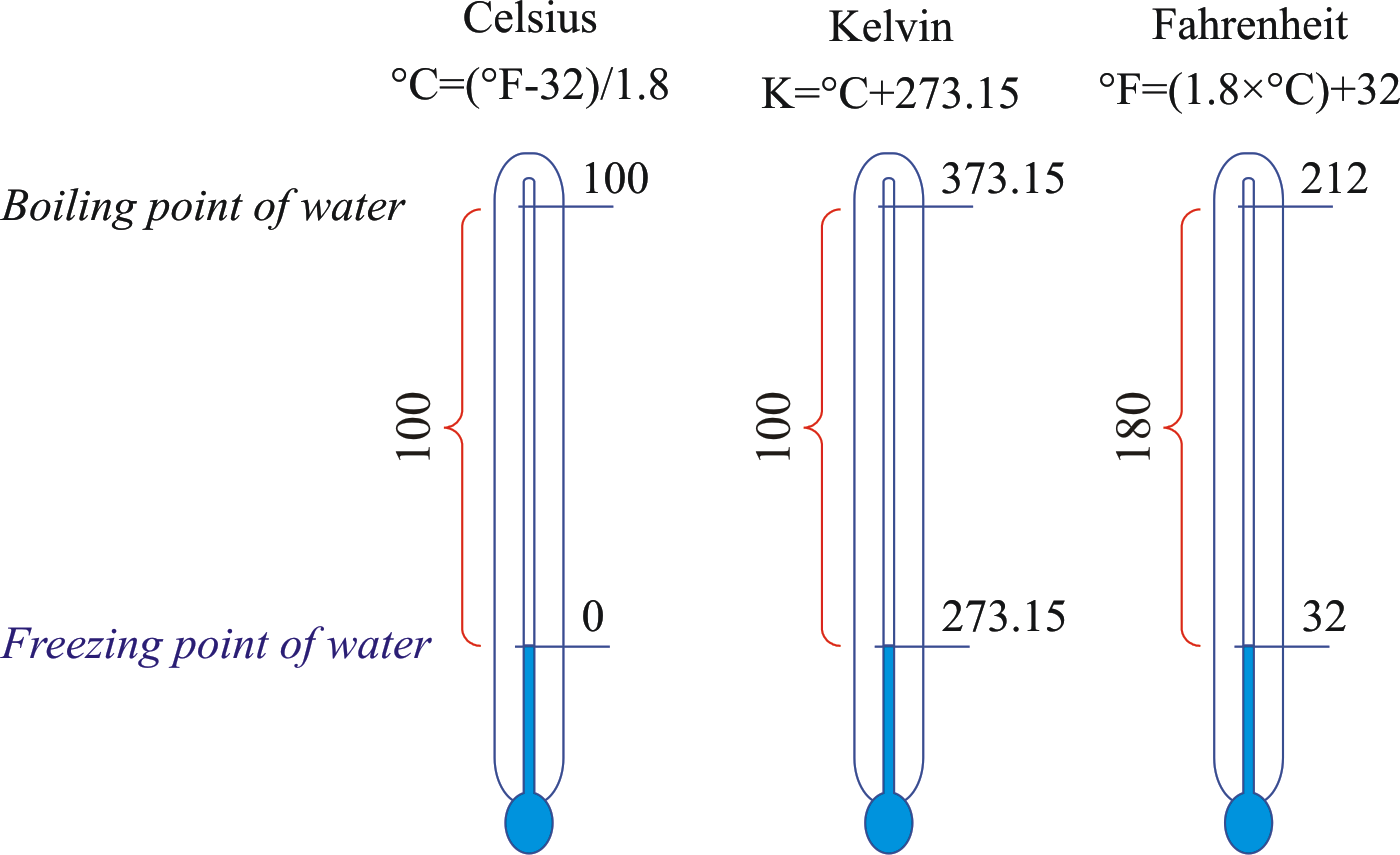
\includegraphics[width=7cm]{fig/temperature_scales.png}
            \newline
            \tiny{Tomado de \href{https://glossary.periodni.com/dictionary.php?en=logaritamska+skala}{aquí}}
        \end{column}
    \end{columns}
\end{frame}

\begin{frame}{Escala de Temperatura}
\begin{table}[]
    \centering
    \begin{tabular}{c|c|c|c}
     \hline
         \hline
        \textbf{Escala} & \textbf{Cero Absoluto} &\textbf{Fusión del hielo} & \textbf{Evaporación} \\
         \hline
         \hline
       \textbf{Kelvin} & 0$ ^{\circ} K$ & 273$ ^{\circ} K$ & 373.2$ ^{\circ} K$ \\
       \textbf{Rankine} & 0$ ^{\circ} R$ & 491.7$ ^{\circ} R$ & 671.7$ ^{\circ} R$ \\
         \textbf{Reamur} & -285.5$ ^{\circ} Re$ & 0$ ^{\circ} Re$ & 80$ ^{\circ} Re$ \\
        \textbf{Centígrada} & -273.2$ ^{\circ} C$ & 0$ ^{\circ} C$ & 100$ ^{\circ} R$ \\
        \textbf{Farenheit} & -459.7$ ^{\circ} F$ & 32$ ^{\circ} R$ & 212.0$ ^{\circ} F$ \\
    \end{tabular}
    \caption{Distintas escalas de temperatura} \cite{cengel2003termodinamica}
    \label{tab:my_label}
\end{table}
\end{frame}

\begin{frame}{Conversión entre escalas}
    \begin{columns}[c, onlytextwidth]
        \begin{column}{0.55\textwidth}
            \begin{itemize}
                \item Valor real de un estimulo: es el que se obtendría con una medición perfecta. Sin embargo este valor es indeterminado y por lo tanto se define por algún tipo de convención. 
                \item Exactitud: es la capacidad de un sensor de dar un resultado cercano al valor real del estímulo medido.
                \item Precisión: es la capacidad de un sensor de dar el mismo resultado cuando se mide el mismo valor de un estimulo bajo las mismas condiciones. 
            \end{itemize}
        \end{column}
        \begin{column}{0.40\textwidth}
            \textbf{Ejemplo}\\[4pt]
            Marca: Amphenol\\[4pt]
            Modelo: NovaSensor NPI-19\\[4pt]
            Estímulo: presión\\[4pt]
            Tipo: piezoresistivo\\[4pt]
            Exactitud estática$^*$: $0.1 \%$ \\[10pt]
            % Exactitud térmica del FSO: $\pm 0.5 \% $\\[4pt]
            % Exactitud térmica del offset: $\pm 0.5 \% $\\[10pt]
            \tiny{* Incluye errores de linealidad, histéresis y repetibilidad}\\
            \tiny{Tomado de \href{https://f.hubspotusercontent40.net/hubfs/9035299/Product\%20Documents/AAS-920-298B-NovaSensor\%20NPI-19-REVISED-061714-web\%20(1).pdf}{aquí}}
        \end{column}
    \end{columns}
\end{frame}

\begin{frame}{Termómetros Industriales}
    \begin{columns}[c, onlytextwidth]
        \begin{column}{0.60\textwidth}
            \begin{itemize}
                \item Repetibilidad: es una medida de la proximidad de la concordancia entre dos mediciones del mismo valor de un estímulo realizadas por la misma persona, con el mismo método e instrumento, bajo las mismas condiciones y en un periodo corto de tiempo. 
                \item Reproducibilidad: es una medida del grado de concordancia entre dos mediciones del mismo valor de un estímulo realizadas por diferentes personas, con el mismo método, con diferentes instrumentos y en un periodo largo de tiempo. 
            \end{itemize}
        \end{column}
        \begin{column}{0.35\textwidth}
            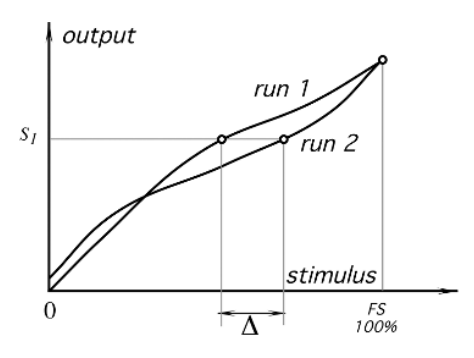
\includegraphics[width=0.9\textwidth]{fig/repeatibility.png}\cite{Fraden_2016}
            \begin{equation*}
                \delta_r = \dfrac{\Delta}{FS}\cdot 100\%
            \end{equation*}
        \end{column}
    \end{columns}
\end{frame}

\begin{frame}{Termopares(Termocuplas)}
    \begin{columns}[c, onlytextwidth]
        \begin{column}{0.55\textwidth}
            \begin{itemize}
                \item Linealidad: es una medida de la proximidad entre la curva de calibración (valores medidos) y una linea recta específica.
                \item Resolución: es el incremento mas pequeño en el valor del estimulo que puede ser medido por el sensor. 
            \end{itemize}
        \end{column}
        \begin{column}{0.40\textwidth}
            \textbf{Ejemplo}\\[4pt]
            Marca: PIHER\\[4pt]
            Modelo: PS2P-LIN\\[4pt]
            Estímulo: posición\\[4pt]
            Tipo: magnetico, efecto Hall\\[4pt]
            Rango del estímulo: $\SI{12}{\milli\meter}$\\[4pt]
            Salida a escala completa (PWM): $10\% (\SI{-6}{\milli\meter}) \sim 90\% (\SI{6}{\milli\meter})$\\[4pt]
            Linealidad: $\pm 1 \%$ \\[4pt]
            Resolución(PWM): $14\,\mathrm{bits}$\\[10pt]
            \tiny{Tomado de \href{https://www.piher.net/pdf/PS2P-LINIntroduction.pdf}{aquí}}
        \end{column}
    \end{columns}
\end{frame}


\begin{frame}{Detector de temperatura por Resistencia (RTD)}
    \begin{columns}[c, onlytextwidth]
        \begin{column}{0.60\textwidth}
            \begin{itemize}
                \item Sensibilidad: es la pendiente de la curva de calibración, sin importar si es constante o no en todo el rango de salida.  
                \item Saturación: es el rango de operación en el que un incremento en el valor del estímulo no produce variaciones en la señal de salida del sensor. 
                \item Banda muerta: es el rango de operación en el que, sin importar el valor del estímulo, la salida es cercana a cero.
            \end{itemize}
        \end{column}
        \begin{column}{0.35\textwidth}
            \textbf{Ejemplo}\\[4pt]
            Marca: Allegro\\[4pt]
            Modelo: ACS723\\[4pt]
            Estímulo: corriente eléctrica\\[4pt]
            Tipo: magnetico, efecto Hall\\[4pt]
            Rango del estímulo: $\SI{10}{\ampere}$\\[4pt]
            Salida a escala completa: $\SI{0.5}{\volt}(\SI{-5}{\ampere}) \sim \SI{4.5}{\volt}(\SI{5}{\ampere})$\\[4pt]
            Sensibilidad: $\SI{400}{\milli\volt/\ampere}$ \\[4pt]
            Saturación: $<\SI{0.5}{\volt}, >\SI{4.5}{\volt}$\\[10pt]
            \tiny{Tomado de \href{https://www.allegromicro.com/-/media/files/datasheets/acs723-datasheet.ashx}{aquí}}
        \end{column}
    \end{columns}
\end{frame}

\begin{frame}{Termistores}
    \begin{columns}[c, onlytextwidth]
        \begin{column}{0.55\textwidth}
            \begin{itemize}
                \item Valor real: es el valor de salida que se obtendría con una medición perfecta. Debido a que esto es imposible de determinar se utiliza una convención para definir el valor real.  
                \item Error absoluto: es la diferencia entre una medición y el valor real. 
                \item Error relativo: es el cociente entre el error absoluto y el valor real
            \end{itemize}
        \end{column}
        \begin{column}{0.40\textwidth}
            \begin{equation*}
                \mathrm{error\,absoluto} = \mathrm{medición} - \mathrm{valor\,real}
            \end{equation*}
            \begin{equation*}
                \mathrm{error\,relativo} = \dfrac{\mathrm{error\,absoluto}}{\mathrm{valor\,real}}
            \end{equation*}
        \end{column}
    \end{columns}
\end{frame}

\begin{frame}{Pirómetros}
    \begin{columns}[c, onlytextwidth]
        \begin{column}{0.55\textwidth}
            \begin{itemize}
                \item Valor real: es el valor de salida que se obtendría con una medición perfecta. Debido a que esto es imposible de determinar se utiliza una convención para definir el valor real.  
                \item Error absoluto: es la diferencia entre una medición y el valor real. 
                \item Error relativo: es el cociente entre el error absoluto y el valor real
            \end{itemize}
        \end{column}
        \begin{column}{0.40\textwidth}
            \begin{equation*}
                \mathrm{error\,absoluto} = \mathrm{medición} - \mathrm{valor\,real}
            \end{equation*}
            \begin{equation*}
                \mathrm{error\,relativo} = \dfrac{\mathrm{error\,absoluto}}{\mathrm{valor\,real}}
            \end{equation*}
        \end{column}
    \end{columns}
\end{frame}

\begin{frame}{Criterios de Selección}
  \begin{table}[]
    \centering
    \begin{tabular}{m{2cm}|m{1.5cm}|m{1.55cm}|m{2cm} | m{1.4cm}}
     \hline
         \hline
        \textbf{Tipo de Sensor} & \textbf{Exactitud} &\textbf{Rango típico} & \textbf{Tiempo de respuesta} & \textbf{Costo} \\
         \hline
         \hline
       \textbf{Termopares} & Baja & -200$ ^{\circ} C$ a 1800$ ^{\circ} C$ & 1 $s$ & Bajo\\
       \textbf{RTD Clase A, Estándar IEC} & Alta & -200$ ^{\circ} C$ a 800$ ^{\circ} C$ & 1-5 $s$ & Alto\\
         \textbf{Termistor NTC} & Alta & -200$ ^{\circ} C$ a 1800$ ^{\circ} C$ & < 1 $s$ & Alto\\
        \textbf{Sensores Infrarrojos} & Mediana & -20$ ^{\circ} C$ a 1370$ ^{\circ} C$ & < 1 $s$ & Bajo \\
    \end{tabular}
    \caption{Comparación entre distintos tipos de sensores}
    \label{tab:Comparacion}
\end{table}
\end{frame}

\begin{frame}{Referencias}
\bibliographystyle{ieeetr}
\footnotesize
\bibliography{comunes/referencias}
\end{frame}

\end{document}